O principal objetivo da modelagem do \textbf{Modelo Entidade-Relacionamento (MER)}, que também é um modelo de dados conceitual de alto nível, é criar um \textbf{esquema conceitual} para o banco de dados da aplicação a ser desenvolvida. Os conceitos utilizados por esse modelo, incluem uma descrição concisa dos requisitos de dados dos usuários e inclui detalhes dos tipos de entidade, relacionamentos e restrições \cite{Navathe:Livro}.

Por não incluirem descrições detalhadas de implementação, esses conceitos normalmente são mais fáceis de entender e podem ser usados parra comunicação com usuários não técnicos. Porém, a maioria dos Sistemas Gerenciadores de Banco de Dados (SGBDs) comerciais utilizam um modelo de dados de implementação - como o modelo de banco de dados relacional ou objeto-relacional- de modo que o esquema conceitual é transformado do modelo de dados de alto nível para o modelo de dados da implementação, etapa conhecida como \textbf{projeto lógico} ou \textbf{mapeamento do modelo de dados} \cite{Navathe:Livro}.

\begin{figure}[H]
	\centering
	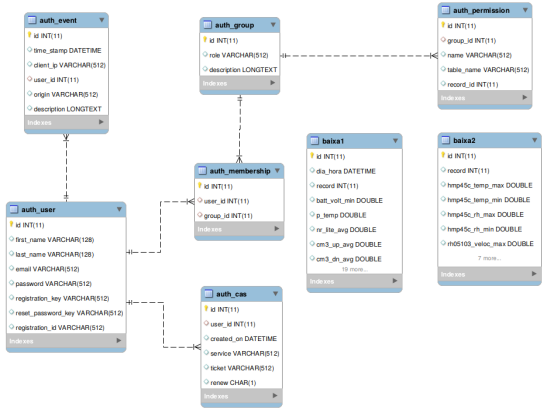
\includegraphics[scale=1.0]{img/mer.png}
	\caption{Módelo Entidade Relacionamento - LabInstru Web.}
	\label{fig:mer}
\end{figure}

na Figura \ref{fig:mer} é mostrado o Modelo Entidade Relaconamento que compõe o banco de dados da plataforma LabInstru Web. Visualmente ao compararmos o Modelo Conceitual e o MER,podemos verificar que ambos possuem semântica bastante similar.
